Algorithms were implemented in separate python libraries to enable re-usability and library sharing among multiple micro services. To ease the development and debugging, visualizations were created and implemented in libraries. Visualization for single agent planning algorithms can be seen on figure \ref{fig:single_agent_path}.

\begin{figure}[H]
    \centering
    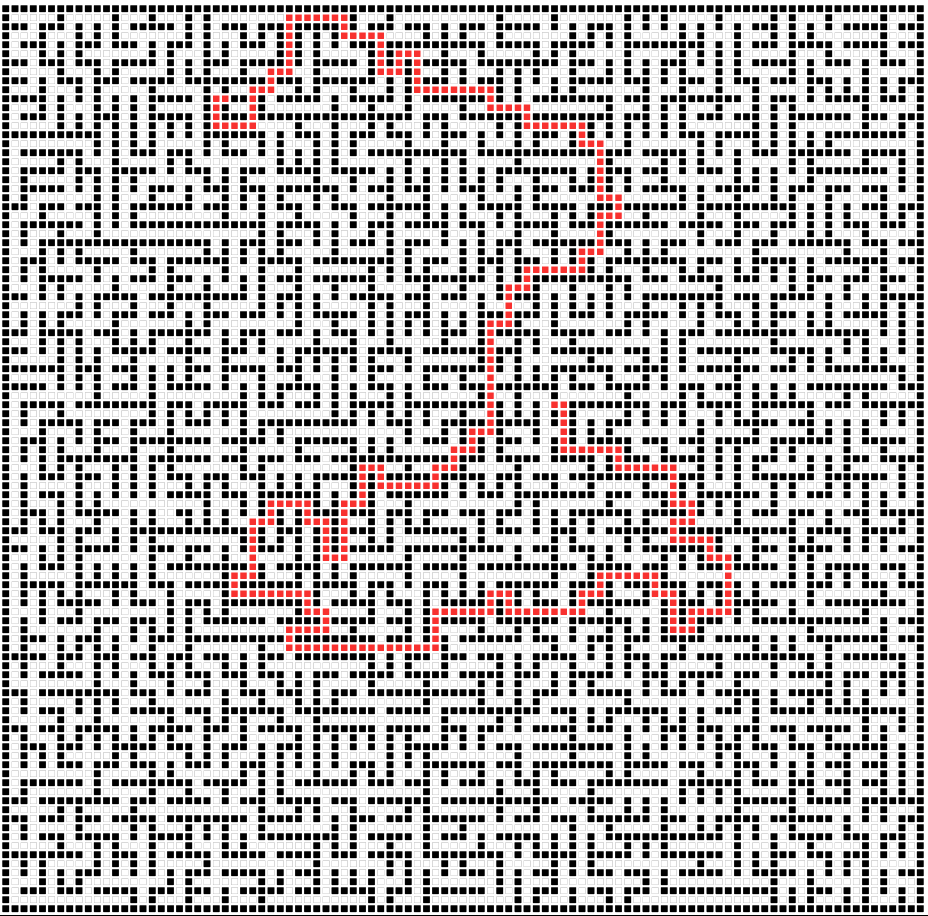
\includegraphics[width=0.6\textwidth]{pictures/single_path_maze.png}
    \caption{ Single agent path planning example} 
    \label{fig:single_agent_path}
\end{figure}


For multi agents algorithms, there are also time consideration and therefore visualizations have to include multiple time frames. To showcase this scenario, example of planed path is shown in figure \ref{fig:multiple_agent_path}. Agents are not colliding and they might choose sub-optimal path to avoid collisions. Start and goal positions are marked with circles, where the agent are marked as squares.

\begin{figure}[H]
    \centering
    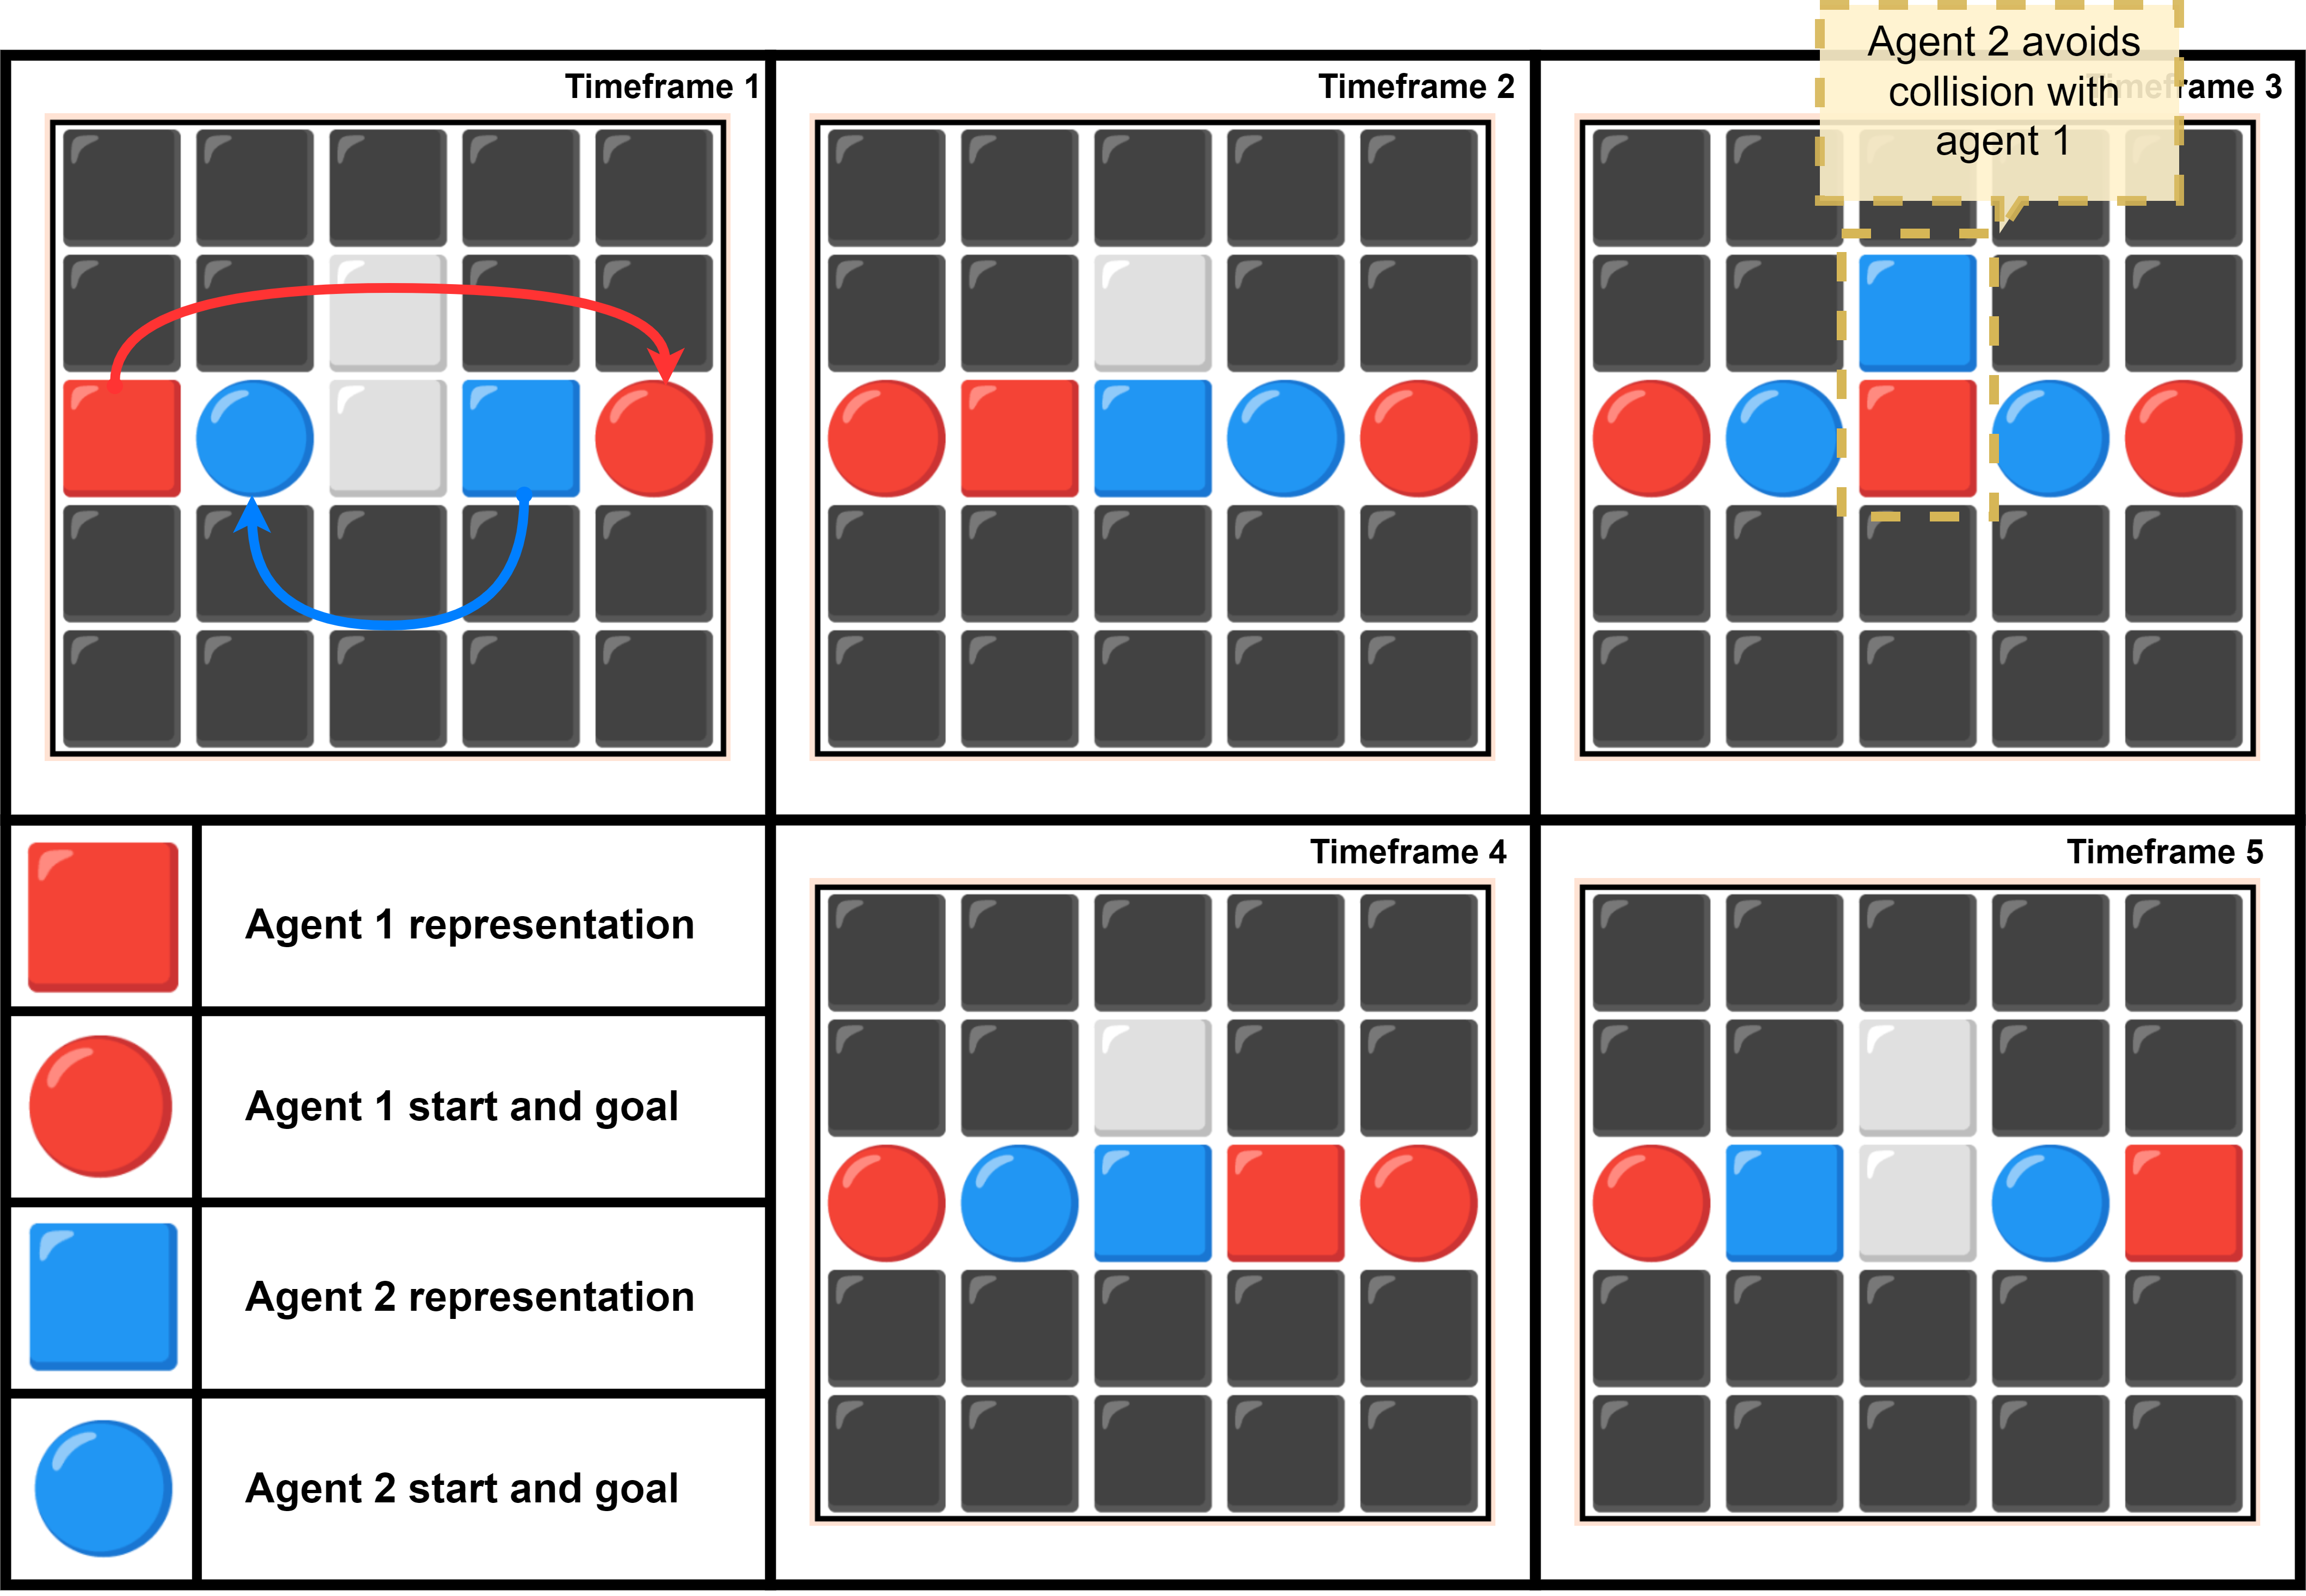
\includegraphics[width=0.9\textwidth]{pictures/example_planning.png}
    \caption{ Example of planned path for multiple agents } 
    \label{fig:multiple_agent_path}
\end{figure}

All libraries are included while building docker image and later imported to the main program. 